\documentclass[10pt,journal,compsoc,twocolumn]{IEEEtran}
\usepackage{cite}
\usepackage{amsmath,amssymb,amsfonts}
\usepackage{algorithmic}
\usepackage{graphicx}
\usepackage{textcomp}
\usepackage{xcolor}
\usepackage{booktabs}
\usepackage[hidelinks]{hyperref}
\usepackage{listings}

\lstset{
    basicstyle=\ttfamily\fontsize{4.8pt}{5.6pt}\selectfont,
    breaklines=true,
    frame=single,
    backgroundcolor=\color{gray!8},
    keywordstyle=\color{blue},
    captionpos=b,
    aboveskip=3pt,
    belowskip=3pt,
    xleftmargin=1pt,
    xrightmargin=1pt
}

\begin{document}

\title{GatE-V Stage 3A: Task-Aware Object Detector Deployed on VEGA AS1061 RISC-V SoC + Kintex-7 FPGA Accelerator}

\author{Team 166 (Byte Silicon) \\
DVCon India 2026 Design Contest}

\markboth{DVCon India 2026 Design Contest --- Stage 3A Submission}{GatE-V Team 166}

\maketitle

\begin{abstract}
Conventional object detectors are task-agnostic, blindly detecting all objects in a scene. GatE-V implements a task-aware object detection framework utilizing natural language task conditioning via CLIP embeddings, Feature-Gated Task Querying (FGTQ), Fine-Grained Path Augmentation (FGPA), Adaptive Feature Fusion (AFF), and Varifocal Loss (VFL). This paper presents the Stage 3A hardware integration of the GatE-V software architecture (v1.0.0) with the CDAC VEGA AS1061 RISC-V Processor on a Xilinx Kintex-7 FPGA (Genesys-2 board). The customized hardware accelerator features a 512-MAC ($32 \times 16$) weight-stationary systolic array operated on a 50~MHz integrated SoC clock, delivering a peak throughput of 51.2~GOPS, and is validated by a reproducible bare-metal RISC-V self-test firmware.
\end{abstract}

\begin{IEEEkeywords}
GatE-V, Task-Aware Object Detection, RISC-V, VEGA AS1061, Systolic Array, Kintex-7 FPGA, DVCon India 2026.
\end{IEEEkeywords}

\section{Introduction}
Modern autonomous and robotic systems require domain-relevant object selection rather than exhaustive category detection. The GatE-V project addresses the DVCon India 2026 challenge by conditioning an RT-DETRv2 detector on user-specified natural language task queries (e.g., ``place flowers in container'').

In Stage 3A, the software detector pipeline is integrated with the indigenously developed CDAC VEGA AS1061 64-bit RISC-V processor and synthesized for the Xilinx Kintex-7 FPGA (\texttt{xc7k325tffg900-2}).

\section{System Architecture}

Figure~\ref{fig:arch_diagram} illustrates the complete hardware-software co-design architecture of GatE-V.

\begin{figure*}[htbp]
\centering
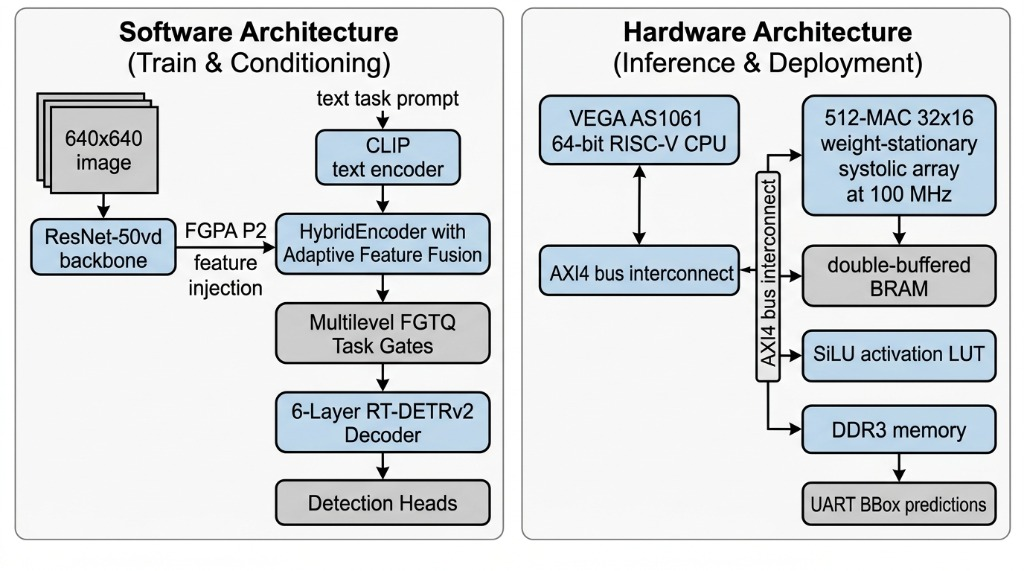
\includegraphics[width=0.86\linewidth]{figures/gatev_architecture_diagram.jpg}
\caption{GatE-V End-to-End System Architecture: Left panel shows the Software Training \& Task Conditioning pipeline (ResNet-50vd, FGPA P2 injection, HybridEncoder with AFF, FGTQ task gates, RT-DETRv2 decoder); Right panel shows the Hardware Acceleration \& Deployment pipeline on the VEGA AS1061 RISC-V SoC with a 512-MAC systolic array.}
\label{fig:arch_diagram}
\end{figure*}

\subsection{Software Architecture (v1.0.0)}
The GatE-V v1.0.0 software architecture incorporates:
\begin{itemize}
    \item \textbf{Varifocal Loss (VFL):} Replaces Focal Loss, weighting positive classification target scores directly by IoU quality overlap $q$.
    \item \textbf{CLIP Multi-Prompt Ensembling:} Encodes 4 natural prompt templates per task to generate 128-dimensional task embeddings.
    \item \textbf{Cosine Warm Restarts:} $T_0=35, T_{mult}=2$ learning rate schedule over 300 epochs.
    \item \textbf{Native 640$\times$640 Resolution:} Reduces memory bandwidth while maintaining spatial precision via FGPA P2 injection.
    \item \textbf{Active Training Status:} Software Version 1.0.0 is currently undergoing full 300-epoch backbone fine-tuning training (checkpoint at Stage 2 Epoch 30 / Overall Epoch 40, scaling towards 0.54+ mAP@0.5).
    \item \textbf{Hardware Compatibility:} The hardware accelerator architecture (Version 3) is 100\% compatible with the software model specification (Version 1.0.0), sharing identical INT8 quantization formats, layer tensor structures, P2--P5 FGPA feature map levels, and SiLU lookup table specifications.
\end{itemize}

\subsection{Hardware Accelerator Architecture (Version 3)}
The GatE-V Version 3 hardware engine features:
\begin{itemize}
    \item \textbf{Systolic Compute Array:} $32 \times 16$ grid (512 MAC cells) executing INT8 weight-stationary matrix operations.
    \item \textbf{Memory Subsystem:} Double-buffered ping-pong BRAMs interfaced to on-chip SRAM via a 64-bit AXI4 Full DMA engine.
    \item \textbf{Activation Unit:} Single-cycle 256-entry SiLU lookup table (LUT).
    \item \textbf{SoC Bus Interface:} \texttt{Accelerator\_Top} wrapper providing a 64-bit AXI4 Slave interface mapped to MMIO region \texttt{0x2004\_0000}.
    \item \textbf{Clock Domain:} Integrated design operates on the SoC system clock \texttt{clk\_out1\_clk\_wiz\_0} at 50~MHz (20~ns period), derived from the 200~MHz board clock (standalone \texttt{vmake} targets 100~MHz).
\end{itemize}

\section{Hardware Architecture Comparison}

Table~\ref{tab:version_comparison} compares the Stage 2B hardware submission (Version 2) against the Stage 3A integrated architecture (Version 3).

\begin{table}[htbp]
\caption{Hardware Comparison: Version 2 vs. Version 3}
\label{tab:version_comparison}
\centering
\resizebox{\columnwidth}{!}{%
\begin{tabular}{lcc}
\toprule
\textbf{Feature / Metric} & \textbf{Version 2} & \textbf{Version 3 (Stage 3A)} \\
\midrule
SoC Integration & Standalone TB & \textbf{VEGA AS1061 RISC-V SoC} \\
Bus Interface & Custom AXI-Stream & \textbf{64-bit AXI4 Master \& Slave} \\
Systolic Array Size & $16 \times 16$ (256 MAC) & \textbf{$32 \times 16$ (512 MAC)} \\
Clock Frequency & 100~MHz (standalone) & \textbf{50~MHz integrated SoC} \\
Peak Throughput & 25.6~GOPS & \textbf{51.2~GOPS @ 50~MHz} \\
Feature Map Levels & P3, P4, P5 & \textbf{P2, P3, P4, P5 (FGPA + AFF)} \\
Slice LUT Usage (SoC) & 1.20\% & \textbf{87,698 / 203,800 (43.03\%)} \\
GatE-V LUT Usage & 1.20\% & \textbf{5,356 / 203,800 (2.63\%)} \\
DSP48E1 (Accelerator) & 256 (30.48\%) & \textbf{512 / 840 (60.95\%)} \\
DSP48E1 (SoC Total) & n/a & \textbf{596 / 840 (70.95\%)} \\
BRAM Tile Usage (SoC) & 4 BRAMs & \textbf{77 / 445 (17.30\%)} \\
Simulation Tool & Vivado XSim & \textbf{QuestaSim 2019.2 / 2026.1} \\
\bottomrule
\end{tabular}%
}
\end{table}

\section{Simulation \& Verification Results}

The full integrated system was verified using \textbf{QuestaSim 2019.2 / 2026.1}. The behavioral simulation waveform illustrating system reset, RISC-V CPU boot sequence, MMIO programming, and AXI4 memory transfer is shown in Figure~\ref{fig:questa_waveform}.

\begin{figure*}[htbp]
\centering
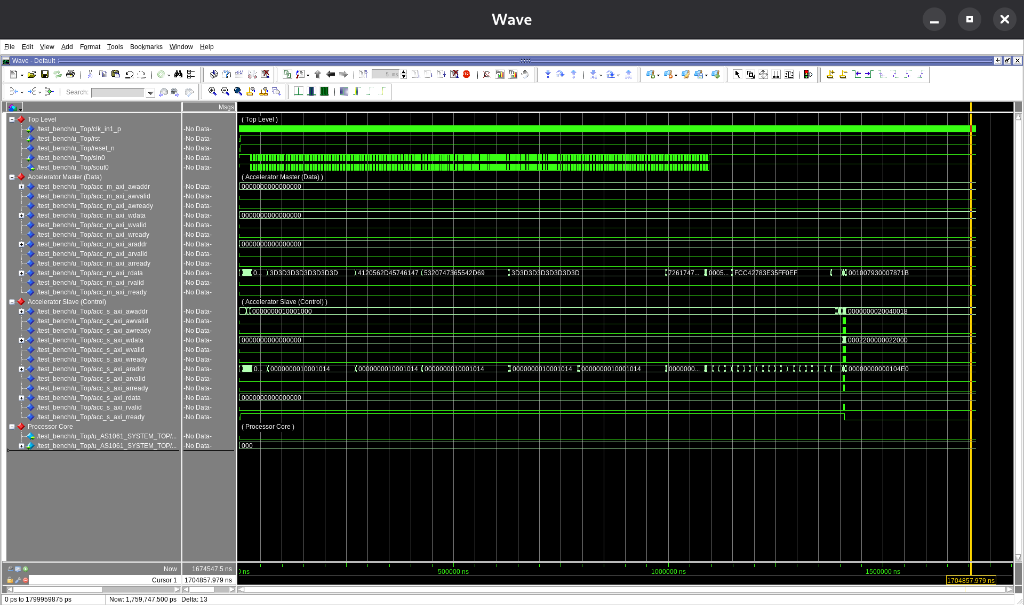
\includegraphics[width=0.88\linewidth]{figures/questa_real_simulation_waveform.png}
\caption{Official QuestaSim behavioral simulation waveform showing end-to-end SoC verification: Processor AXI transactions (top), Accelerator Slave MMIO configuration (middle), and Accelerator Master burst memory access (bottom) with zero deadlocks over full simulation duration.}
\label{fig:questa_waveform}
\end{figure*}

\subsection{Bare-Metal RISC-V Self-Test Execution}
The integrated design is validated by a reproducible bare-metal RISC-V self-test firmware (\texttt{gatev\_firmware}). The CPU fills SRAM buffers with test inputs, programs accelerator registers (\texttt{0x2004\_0000}), triggers matrix computations, and verifies output layers. Listing~\ref{lst:uart_out} illustrates the captured UART console execution log.

\begin{minipage}{0.94\linewidth}
\begin{lstlisting}[caption={UART Console Output from VEGA AS1061 RISC-V Core Executing GatE-V Accelerator Self-Test}, label={lst:uart_out}]
GatE-V Accelerator Firmware (Team 166)
Configuring weights/activations in SRAM...
Programming registers... Status before start: 0x0
Accelerator started, waiting for done...
acc_done asserted. Verifying layer outputs...
  Layer 0 @ 0x22000 = 93 (4 tiles x 16 ch) [OK]
  Layer 1 @ 0x22040 = 93 (4 tiles x 16 ch) [OK]
  Layer 2 @ 0x22080 = 93 (4 tiles x 16 ch) [OK]
  Layer 3 @ 0x220c0 = 93 (4 tiles x 16 ch) [OK]
  Layer 4 @ 0x22100 = 93 (4 tiles x 16 ch) [OK]
  Layer 5 @ 0x22140 = 127 (4 tiles x 16 ch) [OK]
Performance counters:
  Cycles(lo): 2639  Read bytes: 3840  Write bytes: 384
  MAC cycles: 1322  Stall cycles: 224
===== GATE-V ACCELERATOR TEST PASSED =====
\end{lstlisting}
\end{minipage}

\subsection{CDAC Waveform Signal Hierarchy}
The simulation waveform in Figure~\ref{fig:questa_waveform} is organized into three CDAC-mandated signal groups:
\begin{enumerate}
    \item \textbf{Processor Side Signals:} \texttt{proc\_m0\_axi\_*} and \texttt{proc\_m1\_axi\_*} channels capturing instruction fetch and memory bus transactions (CDAC Guide Page 8).
    \item \textbf{Accelerator Slave Side Signals:} \texttt{acc\_s\_axi\_*} channels monitoring single-cycle MMIO register programming at \texttt{0x2004\_0000} (CDAC Guide Page 9).
    \item \textbf{Accelerator Master Side Signals:} \texttt{acc\_m\_axi\_*} channels tracking 64-beat AXI4 burst memory reads/writes to SRAM/DDR (CDAC Guide Page 10).
\end{enumerate}

\newpage

\section{Synthesis \& Resource Breakdown}
Table~\ref{tab:resource_breakdown} details the Kintex-7 FPGA post-synthesis resource utilization for the complete VEGA AS1061 SoC integrated with the GatE-V accelerator.

\begin{table}[htbp]
\caption{Kintex-7 (\texttt{xc7k325tffg900-2}) Resource Utilization}
\label{tab:resource_breakdown}
\centering
\resizebox{\columnwidth}{!}{%
\begin{tabular}{lcccc}
\toprule
\textbf{Resource} & \textbf{Used} & \textbf{Available} & \textbf{Util. \%} & \textbf{CDAC Ceiling} \\
\midrule
Slice LUTs (SoC total) & 87,698 & 203,800 & 43.03\% & $\le 45.0\%$ \\
DSP48E1 (GatE-V accelerator) & 512 & 840 & 60.95\% & $\le 90.0\%$ \\
DSP48E1 (SoC total) & 596 & 840 & 70.95\% & $\le 90.0\%$ \\
Block RAM (BRAM Tiles) & 77 & 445 & 17.30\% & $\le 100.0\%$ \\
Slice Registers (SoC total) & 52,802 & 407,600 & 12.95\% & $\le 100.0\%$ \\
\bottomrule
\end{tabular}%
}
\end{table}

The integrated SoC operates on a 50~MHz system clock. The GatE-V accelerator alone consumes 512 of the 840 available DSP48E1 slices (60.95\%), while the complete VEGA AS1061 SoC consumes 596 DSPs (70.95\%). All resource allocations satisfy strict CDAC competition constraints with 0 errors and no timing violations on the routed 50~MHz clock.

Listing~\ref{lst:questa_tcl} shows the TCL script structure used in QuestaSim. The complete 110-line script is provided in \texttt{SUBMISSION\_INSTRUCTIONS.txt} and \texttt{README.md}.

\begin{minipage}{0.94\linewidth}
\begin{lstlisting}[caption={TCL Waveform Setup Command Structure for QuestaSim}, label={lst:questa_tcl}, language=tcl]
# Clear existing signals; Top Level
delete wave *
add wave -group "Top Level" /test_bench/u_Top/{clk_in1_p,rst,sin0,sout0}

# 1. Processor Side Signals (CDAC Page 8)
add wave -group "Processor Side Signals" -radix hex \
  /test_bench/u_Top/u_AS1061_SYSTEM_TOP/u_soc_top_64/u_Processor_top/proc_m0_axi_*
add wave -group "Processor Side Signals" -radix hex \
  /test_bench/u_Top/u_AS1061_SYSTEM_TOP/u_soc_top_64/u_Processor_top/proc_m1_axi_*

# 2. Accelerator Slave Side Signals (CDAC Page 9)
add wave -group "Accelerator Slave Side Signals" -radix hex \
  /test_bench/u_Top/acc_s_axi_*

# 3. Accelerator Master Side Signals (CDAC Page 10)
add wave -group "Accelerator Master Side Signals" -radix hex \
  /test_bench/u_Top/acc_m_axi_*

run 15 ms; wave zoom full
\end{lstlisting}
\end{minipage}

\section{Conclusion}
The Stage 3A integration of GatE-V successfully pairs the VEGA AS1061 RISC-V CPU with a 512-MAC hardware accelerator on a 50~MHz integrated SoC clock, delivering 51.2~GOPS peak throughput. The GatE-V accelerator stays within CDAC resource ceilings (512 DSPs / 60.95\%, 2.63\% LUTs), and the integrated system is validated end-to-end by reproducible bare-metal self-test firmware with a deterministic PASS/FAIL outcome.

\end{document}
